\newcommand{\proofsketch}{\smallskip\noindent{\bf Proof sketch. }}
\algrenewcommand\algorithmicfunction{\textbf{Machine}}
\newcommand{\bits}{\set{0,1}}
\newcommand{\Ex}{\mathbb{E}}

\renewcommand{\O}{\ensuremath{\mathcal{O}}}
\newcommand{\To}{\rightarrow}
\newcommand{\e}{\epsilon}
\newcommand{\R}{\mathbb{R}}
\newcommand{\N}{\mathbb{N}}
\newcommand{\Z}{\mathbb{Z}}
\newcommand{\logAnd}{\wedge}

\newcommand{\indis}{\mathrel{\overset{\makebox[0pt]{\mbox{\normalfont\tiny c}}}{\approx}}}
\newcommand{\allindis}{\mathrel{\overset{\makebox[0pt]{\mbox{\normalfont\tiny p/s/c}}}{\approx}}}

\newcommand{\cclass}[1]{\mathsf{#1}}
\renewcommand{\P}{\cclass{P}}
\newcommand{\NP}{\cclass{NP}}
\newcommand{\Time}{\cclass{Time}}
\newcommand{\BPP}{\cclass{BPP}}
\newcommand{\Size}{\cclass{Size}}
\newcommand{\Ppoly}{\cclass{P_{/poly}}}
\newcommand{\CSAT}{\ensuremath{\mathsf{CSAT}}}
\newcommand{\SAT}{\ensuremath{\mathsf{3SAT}}}
\newcommand{\IS}{\mathsf{INDSET}}

\newcommand{\inp}{\mathsf{in}}
\newcommand{\outp}{\mathsf{out}}

\newcommand{\Param}{\kappa}
\newcommand{\Adv}{\mathsf{Adv}}
\newcommand{\Supp}{\mathsf{Supp}}

\newcommand{\PRG}{\mathsf{G}}
\renewcommand{\Enc}{\mathsf{Enc}}
\renewcommand{\Dec}{\mathsf{Dec}}
\renewcommand{\sk}{\mathsf{sk}}
\newcommand{\sfC}{\mathsf{C}}
\newcommand{\sfR}{\mathsf{R}}

\newcommand{\eqdef}{\stackrel{\text{\tiny def}}{=}}

\newcommand{\cF}{\mathcal{F}}

\newcommand{\angles}[1]{\langle #1 \rangle}
\newcommand{\iprod}[1]{\angles{#1}}

\newcommand{\Com}{\mathsf{Com}}

% Real vs. Ideal
\newcommand{\RealAdv}{\mathcal{A}}
\newcommand{\IdealAdv}{\mathcal{S}}
\newcommand{\RealVar}{\mathsf{Real}}
\newcommand{\IdealVar}{\mathsf{Ideal}}

% Participating parties
\newcommand{\PartyA}{P_1}
\newcommand{\PartyB}{P_2}
\newcommand{\InputA}{x_1}
\newcommand{\InputB}{x_2}

% Garbling Schemes
\newcommand{\Garble}{\mathsf{Garble}}
\newcommand{\Cir}{C}
\newcommand{\GCir}{\widetilde{C}}
\newcommand{\Lab}{\mathsf{lab}}

% Proof
\newcommand{\Sim}{\mathsf{Sim}}

% GMW

% Misc
\newcommand{\out}{\mathsf{out}}
\newcommand{\Assign}{:=}

\section{zkSNARKs}

In this section, we will overview the fundamentals of zkSNARKs, or Zero-Knowledge Succinct Non-interactive ARguments of Knowledge.

\subsection{Preliminaries}

Before diving into zkSNARKs, let's understand the basic framework we're working with. In cryptography, we often deal with statements of the form ``I know a secret value that satisfies some property.'' For instance, we might want to prove that we know the private key corresponding to a public key, or that we know a solution to a Sudoku puzzle, or that we know a valid password for an account.

To formalize these statements, we use what's called a binary relation $R$. This relation takes two inputs: the public statement $x$ (like a Sudoku puzzle) and the secret witness $w$ (like the solution). $R$ is an efficiently computable binary relation that outputs 1 if the witness $w$ is valid for statement $x$, and 0 otherwise.

For an NP language $\mathcal{L}$, we can say that $x \in \mathcal{L}$ if and only if there exists a witness $w$ such that $R(x, w) = 1$. Conversely, $x \notin \mathcal{L}$ if and only if there does not exist any witness $w$ such that $R(x, w) = 1$. A crucial property is that while finding a valid witness $w$ may be computationally hard (like solving a Sudoku puzzle), verifying the relation $R(x,w)=1$ is always efficient (like checking if a Sudoku solution is valid). This verification can be done in polynomial time.

This framework allows us to express a wide variety of practical problems where we want to prove knowledge of a solution without revealing the solution itself, which is exactly what zkSNARKs will help us achieve.

\subsection{Properties of zkSNARKs}

We now introduce the properties of zkSNARKs. We seek to use zkSNARKs to prove that $x \in L \iff R(x, w) = 1$. Informally, if a prover has $(x, w)$, we must send a proof $\pi$ such that the verifier, who has the instance $x$, can efficiently check that $R(x, w) = 1$. For the purposes of this lecture, we are focusing on non-interactive proof systems. This means that there is no back-and-forth communication between the prover and the verifier, and the verifier can verify the prover's statement in one shot.

Two of the properties of zkSNARKs are common to all proof systems: Correctness ensures that if the statement is true, the prover should always be able to convince the verifier. Soundness ensures that no cheating prover can convince the verifier. However, a correct and sound proof system is not enough for a zkSNARK. Indeed, we could simply achieve this by sending the witness $w$ from the prover to the verifier. We now discuss two properties that are unique to zkSNARKs: Succinctness and Zero knowledge. Succinctness requires that the proof $\pi$ sent by the prover is significantly smaller than the witness $w$. Specifically, the proof size $|\pi|$ must be bounded by $poly(\lambda, \log(|w|))$, where $\lambda$ is the security parameter. This means the proof grows only polylogarithmically with the witness size. Zero knowledge ensures that the proof should not reveal any information about the witness $w$ beyond what can be deduced from the statement being proven. This property is what differentiates zkSNARKs from SNARKs.

The succinctness properties make zkSNARKs incredibly relevant, even for practical applications where we do not care about hiding the witness $w$. This is because the proof size is exponentially more efficient than directly sending the witness $w$ from the prover to the verifier.

\paragraph{Succinctness example.} Let's consider a practical example to illustrate the power of SNARKs' succinctness property. Suppose we have a 1 TB hard disk and want to prove to a verifier that $Hash(hard\text{ }disk) = x$ for some known hash value $x$. We have two options: Without SNARKs, we would need to send the entire 1 TB hard disk to the verifier, who then computes the hash themselves. With SNARKs, we can generate a succinct proof $\pi$ (approximately 1 KB) that proves knowledge of the hard disk contents whose hash equals $x$. Even in scenarios where we do not need to hide the hard disk contents (i.e., zero-knowledge is not required), the SNARK approach is dramatically more efficient in terms of communication complexity: sending a 1 KB proof versus transferring 1 TB of data. This lecture will primarily focus on achieving succinctness, as adding zero-knowledge properties is a relatively straightforward extension once the basic SNARK construction is understood.

\paragraph{How to build SNARKs?} To construct SNARKs, we will follow these key steps. First, we need to find a ``SNARK-friendly'' representation model for NP languages. The example we will use is square span programs. Next, we must show that this model can capture all NP relations, using boolean circuits as an example. Then, we construct the SNARK using cryptographic techniques, specifically employing bilinear groups in our example construction. After that, we prove soundness. Finally, we add zero-knowledge properties. The final SNARK that emerged from this approach is known as Groth16. While we will not cover Groth16 directly, we will study the DFGK14 SNARK, which is conceptually simpler but employs the same fundamental cryptographic ideas.

\subsection{Square Span Programs}

We begin by introducing Square Span Programs (SSPs), which provide a ``SNARK-friendly'' representation for NP languages.

\begin{definition}[Square Span Program]
A square span program $Q$ over a field $\mathbb{F}$ consists of a size parameter $m \in \mathbb{N}$, a degree parameter $d \in \mathbb{N}$, and a set of polynomials $\{v_0(x), v_1(x), \dots, v_m(x), t(x)\}$. Each $v_i(x)$ is a polynomial over $\mathbb{F}$ of degree at most $d$, and $t(x)$ is a polynomial over $\mathbb{F}$ of degree exactly $d$.
\end{definition}

\begin{definition}[SSP Acceptance]
We say that a square span program $Q$ accepts an input $(a_1, \dots, a_\ell) \in \mathbb{F}^\ell$ if and only if there exist values $a_{\ell+1}, \dots, a_m \in \mathbb{F}$ such that $t(x)$ divides $(v_0(x) + \sum_{i=1}^m a_i v_i(x))^2 - 1$. In other words, there exists a polynomial $h(x)$ such that $(v_0(x) + \sum_{i=1}^m a_i v_i(x))^2 - 1 = h(x)t(x)$.
\end{definition}

The values $a_1, \dots, a_\ell$ represent the input to our computation, while $a_{\ell+1}, \dots, a_m$ serve as auxiliary values (similar to a witness in an NP relation). As we will see, this algebraic structure is particularly well-suited for constructing SNARKs. A key property of SSPs is their expressiveness: we can transform any boolean circuit into an equivalent square span program. This transformation will be our next focus.

\subsection{From Boolean Circuits to SSPs}

Consider the boolean circuit in Figure \ref{fig:ssp}. We will transform this circuit into an SSP.

\begin{figure}[h]
  \centering
  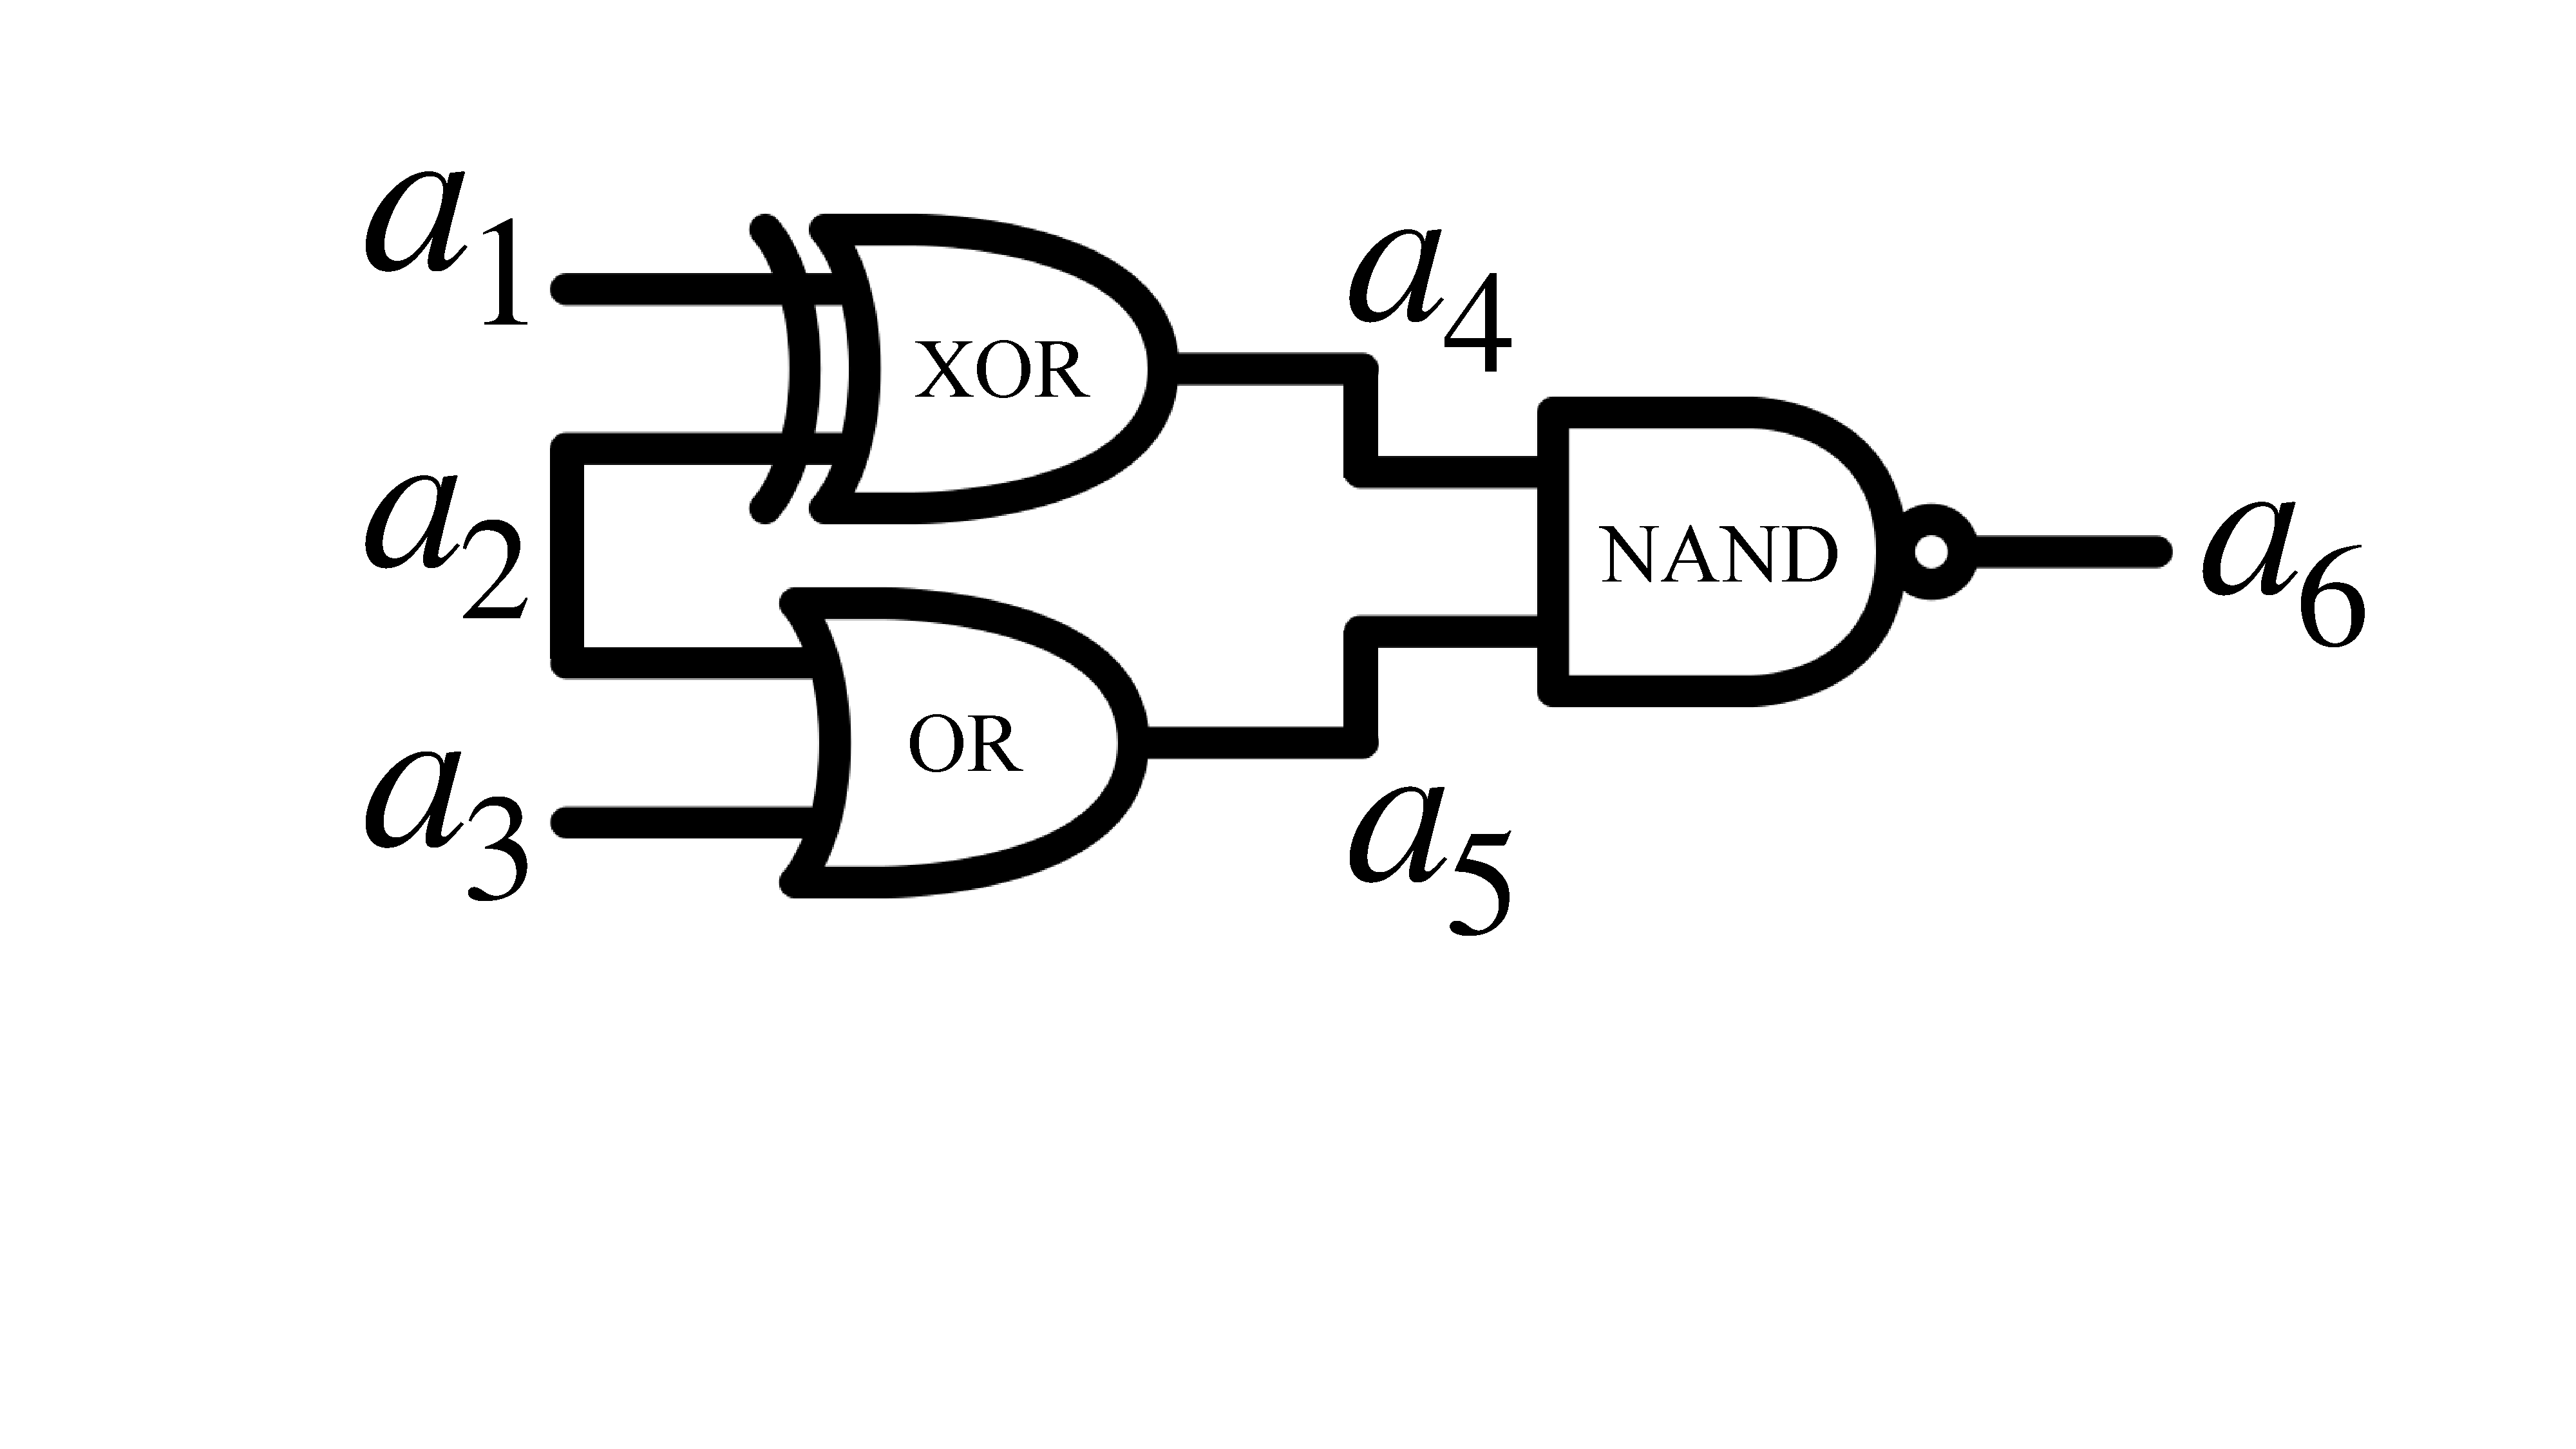
\includegraphics[width=0.4\textwidth]{figures/ssp.pdf}
  \caption{Boolean circuit example for SSP transformation \label{fig:ssp}} 
\end{figure}

First, we formalize the constraints for each gate type. For an XOR gate, the output $a_4$ of inputs $a_1, a_2$ must satisfy $a_1 + a_2 + a_4 \in \{0, 2\}$. For an OR gate, the output $a_5$ of inputs $a_2, a_3$ must satisfy $(1-a_2) + (1-a_3) - 2(1-a_5) \in \{0, 1\}$. For a NAND gate, the output $a_6$ of inputs $a_4, a_5$ must satisfy $a_4 + a_5 - 2(1-a_6) \in \{0, 1\}$.

For the circuit to be satisfiable, all gate constraints must be satisfied, the output constraint $3(1 - a_6) \in \{0, 2\}$ must hold, and all boolean value constraints $a_i \in \{0, 1\}$ for all $i \in \{1,\ldots,6\}$ must be met. To standardize these constraints, we multiply all constraints involving $\{0, 1\}$ by 2 to normalize ranges and combine constraints into a matrix form for $a_1,\ldots,a_6$. Finally, we seek to unify the constraints into a larger matrix that encompasses all the constraints in the whole circuit, where each column represents a single boolean algebra constraint. The resulting constraint matrix $M$ is below, with columns representing the XOR, OR, NAND, and output constraints, respectively:

\[ \begin{pmatrix}
1 & 0 & 0 & 0 & 2 & 0 & 0 & 0 & 0 & 0 \\
1 & -2 & 0 & 0 & 0 & 2 & 0 & 0 & 0 & 0 \\
0 & -2 & 0 & 0 & 0 & 0 & 2 & 0 & 0 & 0 \\
1 & 0 & 2 & 0 & 0 & 0 & 0 & 2 & 0 & 0 \\
0 & 4 & 2 & 0 & 0 & 0 & 0 & 0 & 2 & 0 \\
0 & 0 & 4 & -3 & 0 & 0 & 0 & 0 & 0 & 2
\end{pmatrix} \]

There is also a constant vector $\vec{\delta}$ associated with these constraints:

\[ \vec{\delta} = [0 \; 0 \; -4 \; 3 \; | \; 0 \; 0 \; 0 \; 0 \; 0 \; 0] \]

All constraints must evaluate to elements in $\{0, 2\}^{10}$. 

\paragraph{Generalizing to Arbitrary Circuits.}

Let's now see how we can transform any arbitrary boolean circuit into a Square Span Program. Consider a circuit with $m$ wires and $n$ gates. Our first task is to construct a matrix that captures all the constraints of our circuit. For each gate $k$ in our circuit, we create a column vector $\vec{v_k} = (v_{1k}, v_{2k}, \ldots, v_{mk})^T$ that encodes the gate's constraints. These constraints ensure the gate operates correctly—just as we saw with our XOR, OR, and NAND gates in the previous example.

After encoding all $n$ gates, we add a special column for the output constraint, which takes the form $(0,\ldots,0,-3)^T$. The $-3$ here is somewhat arbitrary; any field element different from 2 would work. We then augment our matrix with a diagonal matrix $D$ where each diagonal entry is 2. This diagonal matrix serves to enforce that all our variables are boolean, a crucial requirement for circuit satisfaction.

To complete our constraint system, we need a constant vector $\vec{\delta} = (\delta_1,\ldots,\delta_n,3,0,\ldots,0)$ where each $\delta_i$ represents the constant term for gate $i$. These constants are chosen from the set $\{0,2\}$, with the exception of the output constraint's constant which is 3.

Let's now see how we can transform any arbitrary boolean circuit into a Square Span Program. Consider a circuit with $m$ wires and $n$ gates. The complete constraint system can be written as:

\[ \begin{pmatrix} a_1 & a_2 & \cdots & a_m \end{pmatrix}
\begin{pmatrix}
v_{11} & v_{12} & \cdots & v_{1n} & 0 & 2 & 0 & \cdots & 0 \\
v_{21} & v_{22} & \cdots & v_{2n} & 0 & 0 & 2 & \cdots & 0 \\
v_{31} & v_{32} & \cdots & v_{3n} & 0 & 0 & 0 & \ddots & 0 \\
\vdots & \vdots & \ddots & \vdots & \vdots & \vdots & \vdots & \ddots & \vdots \\
v_{m1} & v_{m2} & \cdots & v_{mn} & -3 & 0 & 0 & \cdots & 2
\end{pmatrix} + \begin{pmatrix} \delta_1 & \delta_2 & \cdots & \delta_n & 3 & 0 & \cdots & 0 \end{pmatrix} \]

where $(a_1,\ldots,a_m)$ are the wire values (variables we solve for), the first $n$ columns $(v_{ij})$ represent the gate constraints, column $n+1$ is the output constraint $(0,\ldots,0,-3)^T$, the next $m$ columns form the diagonal matrix $D$ with $2$'s on the diagonal, and the constant vector $(\delta_1,\ldots,\delta_m)$ contains $\delta_i \in \{0,2\}$ for $i \leq n$ (gate constraints), $\delta_{n+1} = 3$ (output constraint), and $\delta_i = 0$ for $i > n+1$ (boolean constraints).

Next, we convert these discrete constraints into a polynomial system. We choose distinct field elements $x_1,\ldots,x_d$ (where $d$ is our total number of constraints) and use polynomial interpolation to create our SSP. For each row $i$ of our matrix, we construct a polynomial $v_i(x)$ that evaluates to the $(i,j)$ entry when evaluated at point $x_j$. Similarly, we create a polynomial $v_0(x)$ that interpolates our constant vector $\vec{\delta}$.

The target polynomial $t(x)$ is defined as the product of all linear terms:

\[ t(x) = \prod_{j=1}^d (x-x_j) \]

This polynomial is crucial because it ``zeros out'' exactly at our constraint points. The beauty of this construction is that it transforms our circuit satisfaction problem into an elegant polynomial divisibility question: the circuit is satisfiable if and only if there exist values $(a_1,\ldots,a_m)$ such that:

\[ \left(v_0(x) + \sum_{i=1}^m a_i v_i(x)\right)^2 - 1 = h(x)t(x) \]

for some polynomial $h(x)$.

After converting to a polynomial system, our constraint matrix becomes:

\[ \begin{pmatrix} 
a_1 \\ 
a_2 \\ 
\vdots \\ 
a_m 
\end{pmatrix}^T
\begin{pmatrix}
v_1(x_1) & v_1(x_2) & \cdots & v_1(x_n) & v_1(x_{n+1}) & v_1(x_{n+2}) & 0 & \cdots & 0 \\
v_2(x_1) & v_2(x_2) & \cdots & v_2(x_n) & v_2(x_{n+1}) & 0 & v_2(x_{n+2}) & \cdots & 0 \\
v_3(x_1) & v_3(x_2) & \cdots & v_3(x_n) & v_3(x_{n+1}) & 0 & 0 & \ddots & 0 \\
\vdots & \vdots & \ddots & \vdots & \vdots & \vdots & \vdots & \ddots & \vdots \\
v_m(x_1) & v_m(x_2) & \cdots & v_m(x_n) & v_m(x_{n+1}) & 0 & v_m(x_{n+2}) & \cdots & v_m(x_d)
\end{pmatrix} + 
\begin{pmatrix} v_0(x_1) \\ v_0(x_2) \\ \vdots \\ v_0(x_n) \\ v_0(x_{n+1}) \\ v_0(x_{n+2}) \\ 0 \\ \vdots \\ 0 \end{pmatrix}^T \]

where:
\begin{itemize}
    \item Each $v_i(x_j)$ evaluates to the corresponding matrix entry at point $x_j$
    \item The diagonal entries evaluate to 2 at their respective points
    \item The output constraint column evaluates to $(0,\ldots,0,-3)$ at point $x_{n+1}$
    \item $v_0(x)$ interpolates the constant vector $(\delta_1,\ldots,\delta_n,3,0,\ldots,0)$
\end{itemize}

For any boolean circuit $C$, we can construct an SSP instance $(v_0(x),\ldots,v_m(x),t(x))$ such that $C(x_1,\ldots,x_\ell) = 1$ if and only if there exist values $(a_{\ell+1},\ldots,a_m)$ making the above polynomial division possible.

The correctness of this transformation follows from our construction: each gate's constraints are captured at distinct evaluation points, the boolean nature of our variables is enforced by the diagonal matrix, and the polynomial division condition.




Now, for notational convenience, we define $v_0'(x) = v_0(x) - 1$. 

At each evaluation point $x_j$, our circuit constraints require:
\[ \left(\sum_{i=1}^m a_i v_i(x_j) + v_0'(x_j)\right)^2 = 1 \]

This set of point-wise constraints can be unified into a single polynomial constraint:
\[ \left(\sum_{i=1}^m a_i v_i(x) + v_0'(x)\right)^2 - 1 \equiv 0 \pmod{t(x)} \]

where $t(x) = \prod_{j=1}^d (x - x_j)$ is our target polynomial.

Equivalently, there must exist some polynomial $h(x)$ such that:
\[ \left(\sum_{i=1}^m a_i v_i(x) + v_0'(x)\right)^2 - 1 = h(x)t(x) \]

This is precisely the SSP satisfiability condition. Thus, we have shown that circuit satisfiability is equivalent to the existence of coefficients $a_i$ that satisfy this polynomial divisibility condition.

\subsection{From SSPs to SNARKs}

We'll use bilinear groups to construct our SNARK. Our construction begins with a bilinear group setup:
\[ (\mathbb{F}_p, G_1, G_2, G_T, e, g_1, g_2) \]

The common reference string (CRS) forms the foundation of our construction. It consists of powers of a secret value $\tau$:
\[ \text{CRS} = (bg, g_1^\tau, g_1^{\tau^2}, \dots, g_1^{\tau^d}, g_2^\tau, g_2^{\tau^2}, \dots, g_2^{\tau^d}, g_1^{B v_{\ell + 1}(\tau)}, \dots, g_1^{B v_m(\tau)}, h_2, h_2^B) \]

The core idea of our construction leverages the pairing operation $e$ to verify polynomial equations in the exponent:
\[ e(g_1^{[v_0(x) + \sum_{i=1}^m a_i v_i(x)]}, g_2^{[v_0(x) + \sum_{i=1}^m a_i v_i(x)]}) = e(g_1^{h(x)}, g_2^{t(x)}) \cdot e(g_1, g_2) \]

In our protocol, we distinguish between two types of values:
\begin{itemize}
    \item Statement: $(a_1, \dots, a_\ell)$ - the public inputs
    \item Witness: $(a_{\ell+1}, \dots, a_m)$ - the private values
\end{itemize}

For proof generation, the prover computes four crucial group elements:
\begin{align*}
    \pi_1 &= g_1^{\sum_{i=\ell+1}^m a_i v_i(z)} \\
    \pi_2 &= g_2^{\sum_{i=\ell+1}^m a_i v_i(z)} \\
    \pi_3 &= g_1^{h(z)} \\
    \pi_4 &= g_1^{B\sum_{i=1}^m a_i v_i(z)}
\end{align*}

The verification process consists of two steps. First, the verifier computes intermediate values:
\begin{align*}
    \pi_1' &= g_1^{v_0(z) + \sum_{i=1}^\ell a_i v_i(z)} \cdot \pi_1 \\
    \pi_2' &= g_2^{v_0(z) + \sum_{i=1}^\ell a_i v_i(z)} \cdot \pi_2
\end{align*}

Then, the verifier performs three critical pairing checks:
\begin{align*}
    e(\pi_1', \pi_2') &= e(\pi_3, g_2^{t(z)}) \cdot e(g_1, g_2) \\
    e(\pi_1, g_2) &= e(g_1, \pi_2) \\
    e(\pi_1, h_2^B) &= e(\pi_4, h_2)
\end{align*}

These pairing equations serve distinct purposes in ensuring the proof's validity. The first check confirms that the SSP is satisfied by verifying the polynomial equation in the exponent. The second check ensures consistency between the prover's elements in groups $G_1$ and $G_2$. The final check prevents malformed group elements by verifying they were properly constructed using the CRS values.

\subsection{Soundness}

Due to the non-interactive nature of our protocol, we cannot rely on black-box extraction for our security proofs. Instead, we require a non-black-box extractor with access to the prover's code, which is acceptable within our security model.

The soundness guarantees of SNARKs, including our SSP SNARK construction, differ from traditional cryptographic protocols. They necessarily rely on non-falsifiable assumptions or the random oracle model (ROM).

Non-falsifiable assumptions represent a unique class of cryptographic assumptions. Informally, given $(g, g^\alpha)$, these assumptions state that no adversary can output a pair $(g^x, (g^x)^\alpha)$ without actually ``knowing'' the exponent $x$. The term ``non-falsifiable'' stems from the fact that these assumptions make claims about what an adversary must know, rather than just what it can or cannot compute.

Our first attempt at formalizing soundness states that for every probabilistic polynomial-time (PPT) adversary $\mathcal{A}$, there exists a PPT extractor $E_\mathcal{A}$ such that:
\[ \Pr[(v_1, v_2) \gets \mathcal{A}(g, g^\alpha, z), x \gets E_\mathcal{A}(g, g^\alpha, z) : v_2 = v_1^\alpha \land v_1 \neq g^x] = negl(\lambda) \]

This probability involves three key components:
\begin{itemize}
    \item $z$ represents auxiliary information available to the adversary
    \item $\lambda$ denotes the security parameter
    \item $negl(\lambda)$ represents a negligible function
\end{itemize}

Recent research has revealed limitations in this initial formulation. Specifically, certain obfuscated programs, when provided as auxiliary input $z$, enable adversaries to produce valid pairs $(v_1, v_2)$ while preventing the extractor $E_\mathcal{A}$ from determining $x$ due to the complexity of reverse-engineering the obfuscated program.

\subsubsection{Knowledge Soundness Definition}

To address these limitations, we've developed a more robust formulation for our SNARK construction. For all relations $R \in \mathcal{R}$, benign auxiliary information $z \in \mathcal{Z}$, and non-uniform adversaries $\mathcal{A}$, there exists a non-uniform PPT extractor $E_\mathcal{A}$ such that for all benign $z \in \mathcal{Z}$:
\[ \begin{aligned}
&\Pr[((v_1, v_2); c_0, \dots, c_d) \gets (\mathcal{A} \| E_\mathcal{A})(bg, g_1, g_2, \dots, g_2^{\tau^d}, z) : \\
&\quad e(v_1, g_2) = e(g_1, v_2) \land v_1 \neq g_1^{\sum_{i=0}^d c_i \tau^i}] = negl(\lambda)
\end{aligned} \]

This refined definition captures several crucial aspects: the adversary and extractor share access to the bilinear group setup and CRS, the extractor must produce coefficients $c_i$ explaining the adversary's output, the auxiliary information must be ``benign'' (excluding problematic cases like obfuscated programs), and the probability of adversarial success without the extractor finding a valid witness must be negligible.

While this non-falsifiable assumption is stronger than traditional cryptographic assumptions, it appears to be necessary for constructing efficient SNARKs using current techniques.

\subsubsection{Knowledge Assumption}

We now formalize the knowledge assumption d-PKE (power knowledge of exponent).

For every non-uniform PPT adversary $\mathcal{A}$ there exists a non-uniform PPT extractor $E_\mathcal{A}$ such that for every ``benign'' $z$:

$$\Pr [\mathcal{A} || E_\mathcal{A} (bg, g_1^\tau, g_1^{\tau^2}, \dots, g_1^{\tau^d}, g_2^\tau, g_2^{\tau^2}, \dots, g_2^{\tau^d}, z)$$
$$\rightarrow (v_1, v_2; c_0, \dots, c_d) : e(v_1, g_2) = e(g_1, v_2) \land v_1 \neq g_1^{\sum_{i=0}^d c_i \tau^i}] = negl(\lambda)$$

This is basically saying that if the adversary can output a valid pair $(v_1, v_2)$ then the extractor can output a polynomial with coefficients $c_0, \dots, c_d$ such that $v_1 = g_1^{\sum_{i=0}^d c_i \tau^i}$. Observe this assumption is very close to what we actually construct in the SNARK.

We now show a sketch of the knowledge soundness proof.

Assuming a knowledge-sound adversary $\mathcal{A}$, we are going to construct $\mathcal{A}'$ as follows:

$$\mathcal{A}'(bg, \{g_1^{z^i}\}_{i=0}^d, \{g_2^{z^i}\}_{i=0}^d, z' = (z || \{g_1^{B v_i(\tau)}\}_{i=\ell+1}^m h_1, h_2^B)) \rightarrow (a_1, \dots, a_\ell, a_{\ell+1}, \dots, a_m)$$

We give the rest of the CRS of the SNARK to the adversary inside of the auxiliary input $z'$. Then, this adversary runs the adversary of the knowledge soundness assumption as follows:

$$\mathcal{A}(R, z, crs) \rightarrow (\pi_1, \pi_2, \pi_3, \pi_4, (a_1, \dots, a_\ell))$$

and outputs $v_1 = \pi_1 g_1^{v_0(z) + \sum_{i=1}^\ell a_i v_i(z)}$, $v_2 = \pi_2 g_2^{v_0(z) + \sum_{i=1}^\ell a_i v_i(z)}$ where $e(v_1, g_2) = e(g_1, v_2)$.

There is an extractor $E_\mathcal{A}'$ that can output $c_0, \dots, c_d$ such that $v_1 = g_1^{\sum_{i=0}^d c_i \tau^i}$.

So note that if we have the extractor $E_\mathcal{A}$ and $a_{\ell+1}, \dots, a_m$ for the witness, and $v_1 = g_1^{F(z)}$, then we can output $(a_1, \dots, a_\ell, a_{\ell+1}, \dots, a_m)$.

We now construct the extractor $E_\mathcal{A}$ for knowledge soundness. The extractor is given $a_{\ell+1}, \dots, a_m$. $v_1 = g_1^F(\tau)$ where $F(x) = \sum_{i=0}^d c_i x^i$.

In order for this extractor to be able to extract the actual witness of the relation, we need two things:
\begin{enumerate}
    \item $(f(x))^2 - 1$ is divisible by $t(x)$, which is also known as the $d$-Target Group Strong Diffie-Hellman assumption.
    \item $f_{wit}(x) := f(x) - v_0(x) - \sum_{i=1}^\ell a_i v_i(x)$ is in the span of $\{v_i\}_{i=\ell+1}^m$, which is also known as the $d$-Power Diffie-Hellman assumption.
\end{enumerate}

So if we can write $f(x) = \sum_{i=0}^d c_i x^i = v_0(x) + \sum_{i=1}^\ell a_i v_i(x)$ and $(f(x))^2 - 1$ is divisible by $t(x)$. Given this then $(a_\ell+1, \dots, a_m)$ is a valid witness for the relation and so we can say that there exists a witness $a_{\ell+1}, \dots, a_m$ such that $f_{wit}(x) = \sum_{i=\ell+1}^m a_i v_i(x)$.